\section{Introduction}
\label{sec:intro}

The emergence of large language models (\emph{LLMs}) like GPT~\cite{openai2023gpt4,brown2020language} and PaLM~\cite{chowdhery2022palm} have enabled new applications such as programming assistants~\cite{copilot, chen2021evaluating} and universal chatbots~\cite{chatgpt, bard} that are starting to profoundly impact our work and daily routines. Many cloud companies~\cite{openaiapi, amazonbedrock} are racing to provide these applications as hosted services. However, running these applications is very expensive, requiring a large number of hardware accelerators such as GPUs. According to recent estimates, processing an LLM request can be 10$\times$ more expensive than a traditional keyword query~\cite{chat-cost}.
Given these high costs, increasing the throughput---and hence reducing the cost per request---of \emph{LLM serving} systems is becoming more important.

{\let\thefootnote\relax\footnote{{$^*$Equal contribution.}}\addtocounter{footnote}{-1}} At the core of LLMs lies an autoregressive Transformer model~\cite{vaswani2017attention}. 
This model generates words (tokens), \emph{one at a time}, based on the input (prompt) and the previous sequence of the output's tokens it has generated so far.
For each request, this expensive process is repeated until the model outputs a termination token.
This sequential generation process makes the workload \emph{memory-bound}, underutilizing the computation power of GPUs and limiting the serving throughput.

\begin{figure}
    \centering
    \begin{subfigure}[c]{0.40\columnwidth}
    \centering
    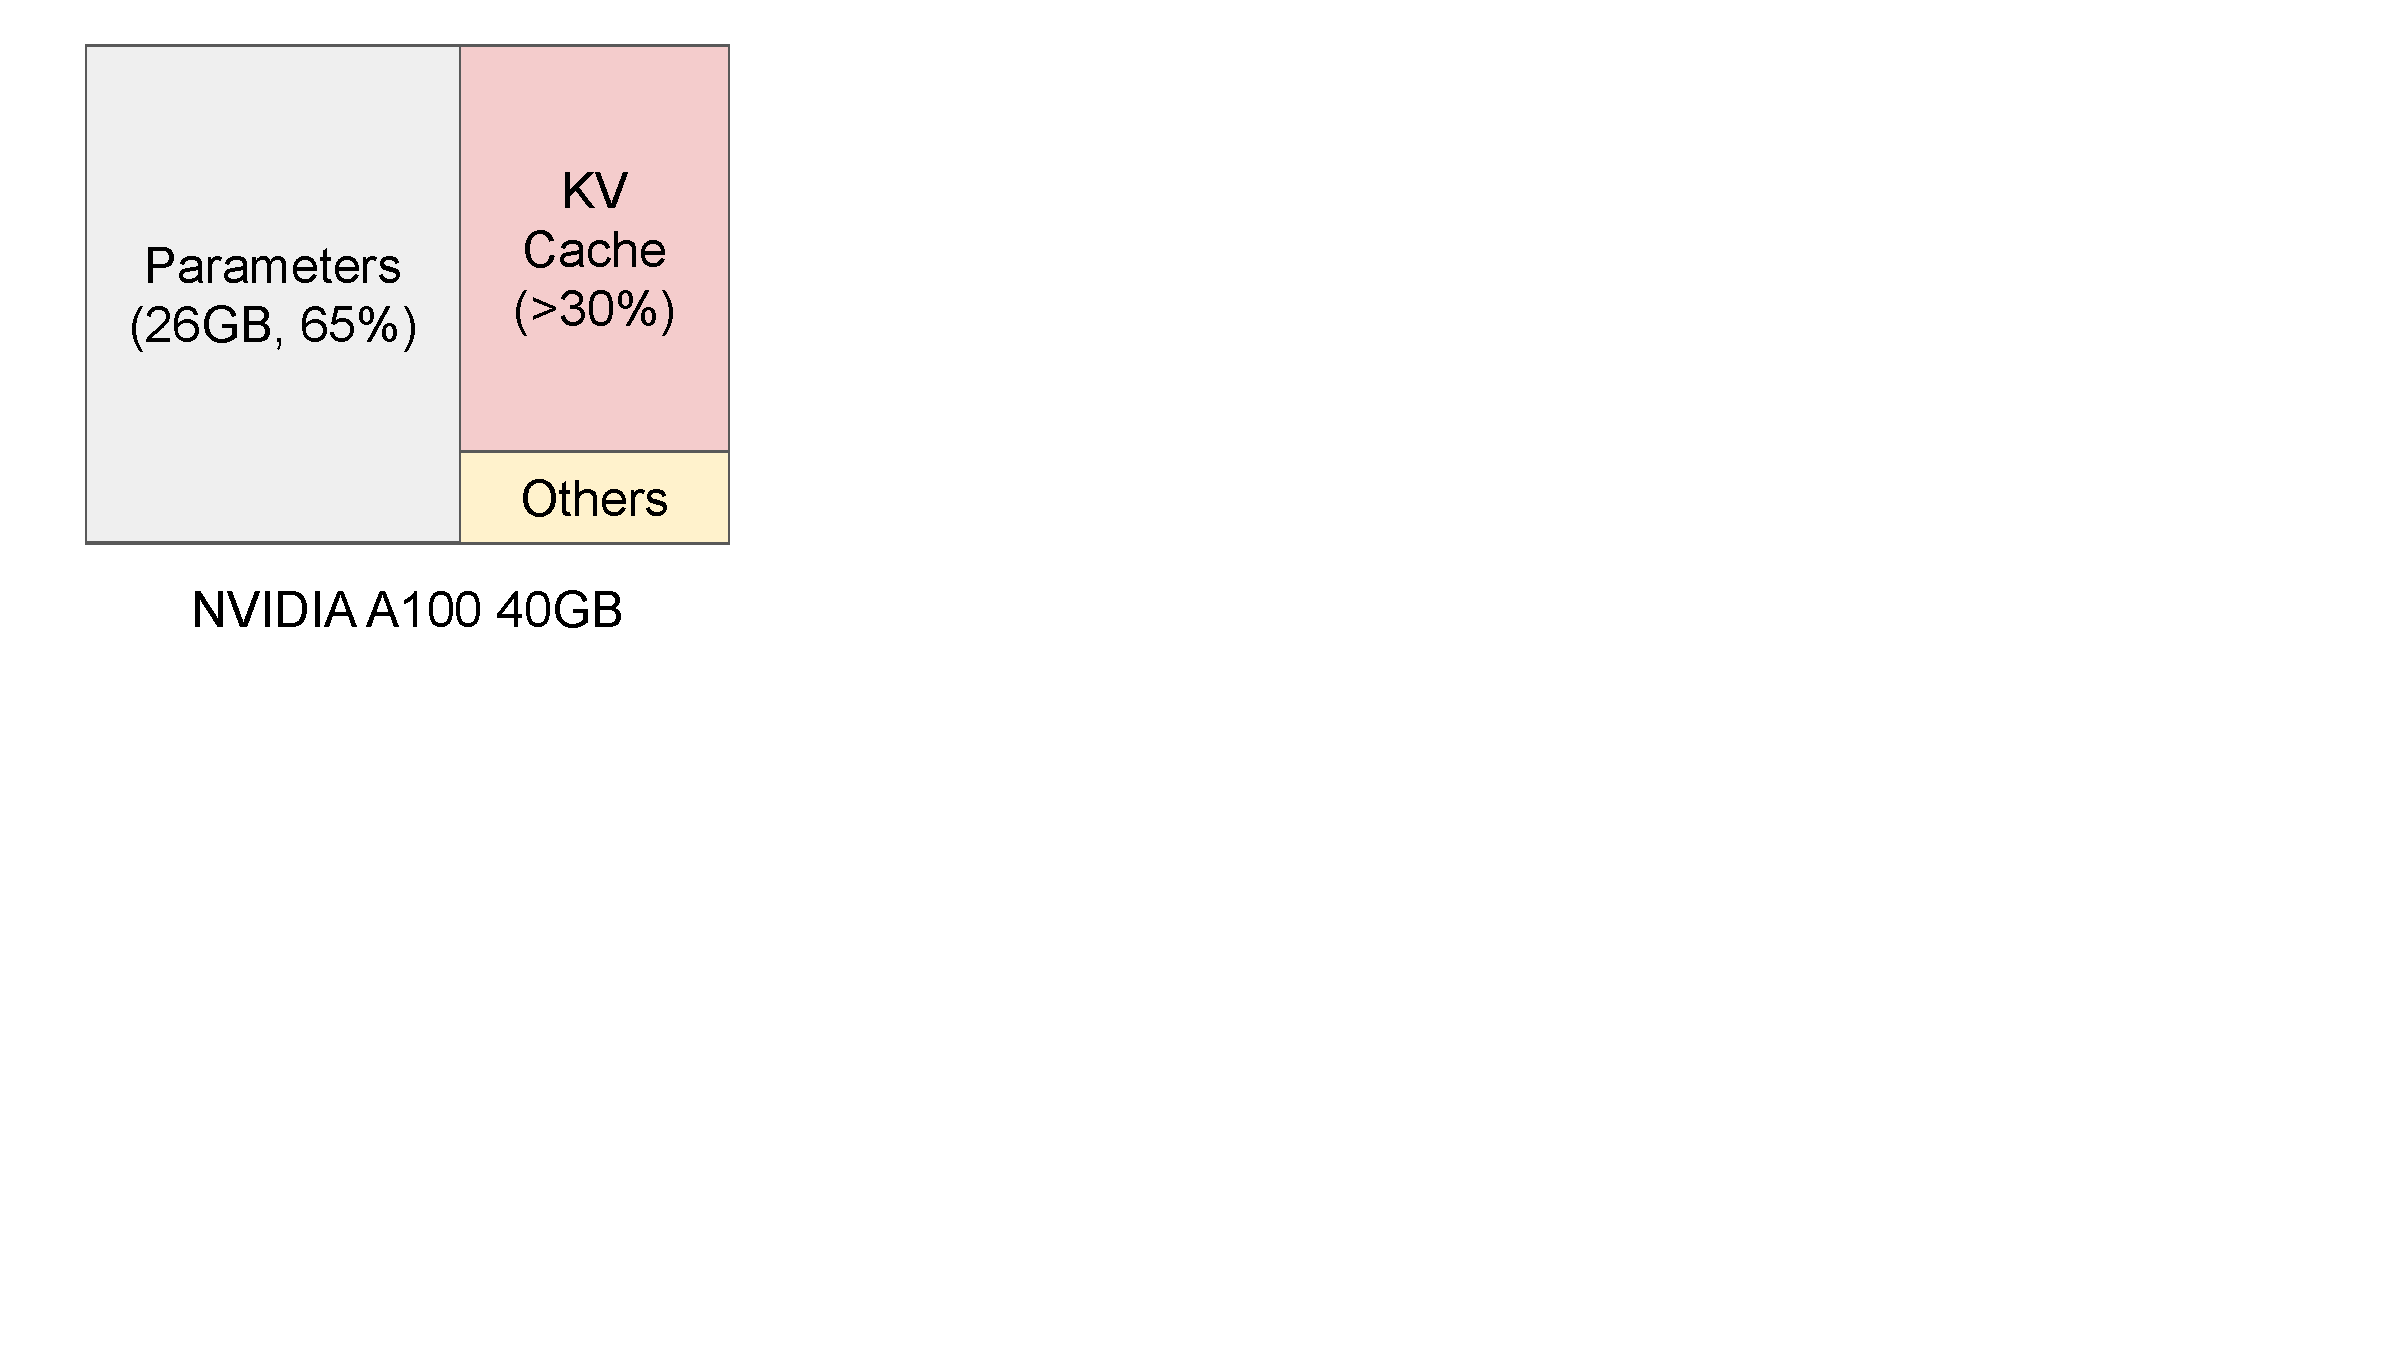
\includegraphics[width=\columnwidth]{figures/memory-distribution.pdf}  
    \end{subfigure}
    \hfil
    \begin{subfigure}[c]{0.50\columnwidth}
    \centering
    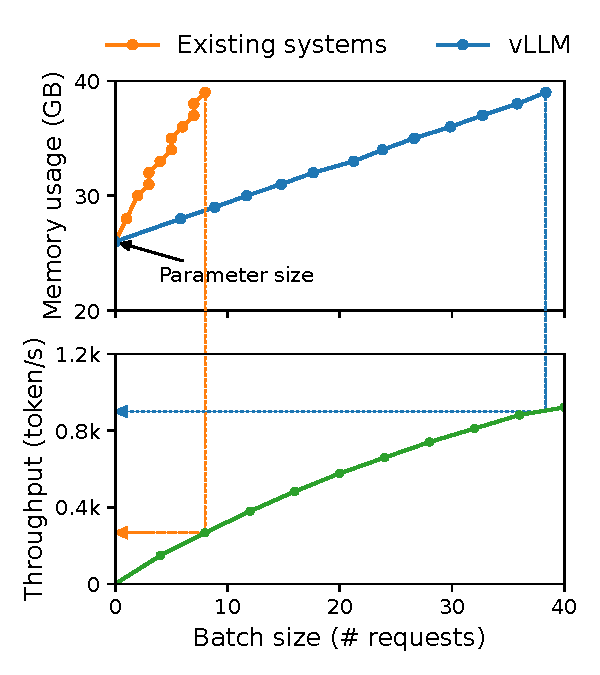
\includegraphics[width=\columnwidth]{figures/memory_batchsize.pdf}
    \end{subfigure}
    \vspace{-10pt}
    \caption{\emph{Left:} Memory layout when serving an LLM with 13B parameters on NVIDIA A100. The parameters (gray) persist in GPU memory throughout serving. The memory for the KV cache (red) is (de)allocated per serving request. A small amount of memory (yellow) is used ephemerally for activation. 
    \emph{Right:}
    \sys smooths out the rapid growth curve of KV cache memory seen in existing systems~\cite{nvidiaft,yu2022orca}, leading to a notable boost in serving throughput.}
    \label{fig:motivation}
\end{figure}

Improving the throughput is possible by batching multiple requests together.
However, to process many requests in a batch, the memory space for each request should be efficiently managed.
For example, Fig.~\ref{fig:motivation} (left) illustrates the memory distribution for a 13B-parameter LLM on an NVIDIA A100 GPU with 40GB RAM.
Approximately 65\% of the memory is allocated for the model weights, which remain static during serving.
Close to 30\% of the memory is used to store the dynamic states of the requests.
For Transformers, these states consist of the key and value tensors associated with the attention mechanism, commonly referred to as \emph{KV cache}~\cite{pope2022efficiently}, which represent the context from earlier tokens to generate new output tokens in sequence.
The remaining small percentage of memory is used for other data, including activations – the ephemeral tensors created when evaluating the LLM.
Since the model weights are constant and the activations only occupy a small fraction of the GPU memory, the way the KV cache is managed is critical in determining the maximum batch size.
When managed inefficiently, the KV cache memory can significantly limit the batch size and consequently the throughput of the LLM, as illustrated in Fig.~\ref{fig:motivation} (right).

In this paper, we observe that existing LLM serving systems~\cite{yu2022orca,nvidiaft} fall short of managing the KV cache memory efficiently.
This is mainly because they store the KV cache of a request in contiguous memory space, as most deep learning frameworks~\cite{paszke2019pytorch, olston2017tensorflow} require tensors to be stored in contiguous memory.
However, unlike the tensors in the traditional deep learning workloads, the KV cache has unique characteristics: it dynamically grows and shrinks over time as the model generates new tokens, and its lifetime and length are not known a priori.
These characteristics make the existing systems' approach significantly inefficient in two ways:

\begin{figure}[t]
    \centering
    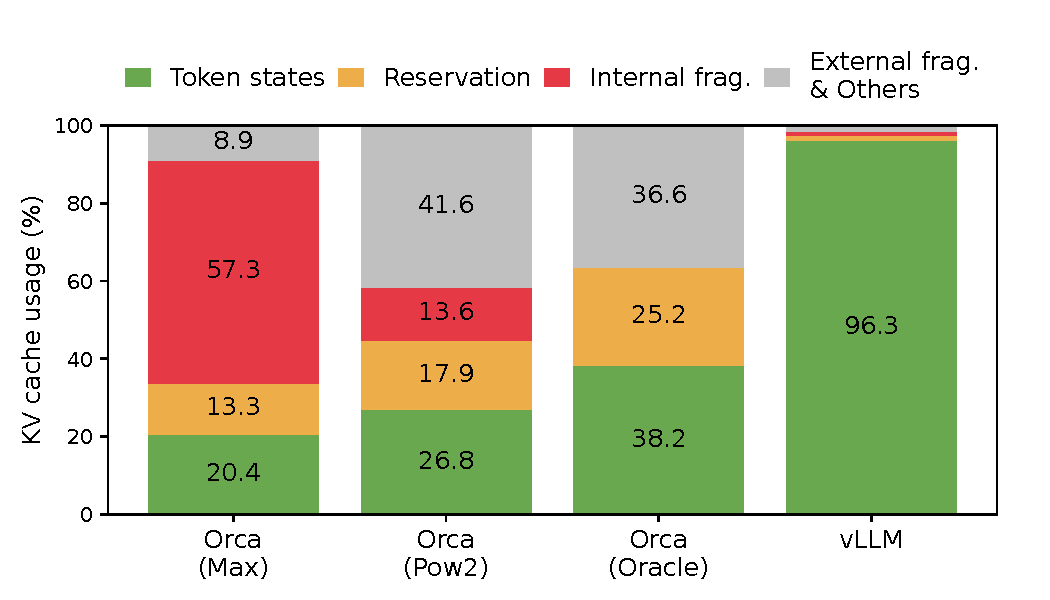
\includegraphics[width=\columnwidth]{figures/experiments/memory_breakdown.pdf}
    \caption{Average percentage of memory wastes in different LLM serving systems during the experiment in \S\ref{sec:eval:basic-sampling}.}
    \label{fig:memory-waste-percentage}
\end{figure}

First, the existing systems~\cite{yu2022orca,nvidiaft} suffer from internal and external memory fragmentation.
To store the KV cache of a request in contiguous space, they \emph{pre-allocate} a contiguous chunk of memory with the request's maximum length (e.g., 2048 tokens).
This can result in severe internal fragmentation, since the request's actual length can be much shorter than its maximum length (e.g., Fig.~\ref{fig:dataset-length-dist}).
Moreover, even if the actual length is known a priori, the pre-allocation is still inefficient: As the entire chunk is reserved during the request's lifetime, other shorter requests cannot utilize any part of the chunk that is currently unused.
Besides, external memory fragmentation can also be significant, since the pre-allocated size can be different for each request.
Indeed, our profiling results in Fig.~\ref{fig:memory-waste-percentage} show that only 20.4\% - 38.2\% of the KV cache memory is used to store the actual token states in the existing systems.

Second, the existing systems cannot exploit the opportunities for memory sharing.
LLM services often use advanced decoding algorithms, such as parallel sampling and beam search, that generate multiple outputs per request.
In these scenarios, the request consists of multiple sequences that can partially share their KV cache.
However, memory sharing is not possible in the existing systems because the KV cache of the sequences is stored in separate contiguous spaces.

To address the above limitations, we propose \emph{\tech}, an attention algorithm inspired by the operating system's (OS) solution to memory fragmentation and sharing: \emph{virtual memory with paging}.
\tech divides the request's KV cache into blocks, each of which can contain the attention keys and values of a fixed number of tokens.
In \tech, the blocks for the KV cache are not necessarily stored in contiguous space.
Therefore, we can manage the KV cache in a more flexible way as in OS’s virtual memory: one can think of blocks as pages, tokens as bytes, and requests as processes.
This design alleviates internal fragmentation by using relatively small blocks and allocating them on demand.
Moreover, it eliminates external fragmentation as all blocks have the same size.
Finally, it enables memory sharing at the granularity of a block, across the different sequences associated with the same request or even across the different requests.

In this work, we build \emph{\sys}, a high-throughput distributed LLM serving engine on top of \tech that achieves near-zero waste in KV cache memory.
vLLM uses block-level memory management and preemptive request scheduling that are co-designed with \tech.
\sys supports popular LLMs such as GPT~\cite{brown2020language}, OPT~\cite{zhang2022opt}, and LLaMA~\cite{touvron2023llama} with varying sizes, including the ones exceeding the memory capacity of a single GPU.
Our evaluations on various models and workloads show that \sys improves the LLM serving throughput by 2-4$\times$ compared to the state-of-the-art systems~\cite{yu2022orca,nvidiaft}, without affecting the model accuracy at all.
The improvements are more pronounced with longer sequences, larger models, and more complex decoding algorithms (\S\ref{sec:one-sequence-decoding-example}).
In summary, we make the following contributions:
\begin{CompactItemize}
    \item We identify the challenges in memory allocation in serving LLMs and quantify their impact on serving performance.
    \item We propose \tech, an attention algorithm that operates on KV cache stored in non-contiguous paged memory, which is inspired by the virtual memory and paging in OS.
    \item We design and implement \sys, a distributed LLM serving engine built on top of \tech.
    \item We evaluate \sys on various scenarios and demonstrate that it substantially outperforms the previous state-of-the-art solutions such as FasterTransformer~\cite{nvidiaft} and Orca~\cite{yu2022orca}.
\end{CompactItemize}
